\section{Resultados}
\label{sec:results}

Esta seção organiza os resultados em dois blocos independentes.
Primeiro, discute-se o comportamento dos métodos clássicos em termos de qualidade, custo, robustez ao ruído e relação com a entropia local.
Em seguida, analisa-se o bloco de aprendizado profundo, focado na comparação interna entre arquiteturas treinadas no domínio Sentinel-2.
Essa separação é parte do rigor interpretativo do trabalho, pois evita atribuir a diferenças algorítmicas aquilo que pode decorrer de diferenças de escopo experimental.

\subsection{Resultados dos Métodos Clássicos}

O panorama global dos métodos clássicos é apresentado na \Cref{tab:global-scoreboard-classical}.
O primeiro aspecto que a tabela evidencia é a ausência de dominância universal.
Não existe um método que lidere simultaneamente em qualidade radiométrica, preservação estrutural, coerência espectral e custo computacional.
Em lugar de um vencedor absoluto, observa-se um grupo relativamente pequeno de métodos fortes, com perfis distintos e compensações claras entre desempenho e viabilidade prática.

\begin{table*}[htbp]
\centering
\caption{Placar global multi-métrica dos métodos clássicos por nível de ruído (mediana e IC95\%). \textbf{Negrito}: melhor por métrica dentro do grupo.}
\label{tab:global-scoreboard-classical}
\footnotesize
\resizebox{\linewidth}{!}{%
\begin{tabular}{llccccc}
\toprule
Tipo & Método & PSNR (dB) $\uparrow$ & SSIM $\uparrow$ & RMSE $\downarrow$ & SAM $\downarrow$ & ERGAS $\downarrow$ \\
\midrule
\multicolumn{7}{l}{\textbf{Nível de ruído: todos os níveis de ruído}} \\
Clássico & kriging & $\mathbf{20.90_{\pm 1.355}}$ & $0.57_{\pm 0.038}$ & $\mathbf{0.09_{\pm 0.014}}$ & $\mathbf{6.27_{\pm 0.772}}$ & $\mathbf{31.98_{\pm 3.236}}$ \\
Clássico & rbf & $20.40_{\pm 1.255}$ & $0.58_{\pm 0.031}$ & $0.10_{\pm 0.014}$ & $7.69_{\pm 0.825}$ & $33.86_{\pm 2.915}$ \\
Clássico & spline & $20.40_{\pm 1.255}$ & $0.58_{\pm 0.031}$ & $0.10_{\pm 0.014}$ & $7.69_{\pm 0.825}$ & $33.86_{\pm 2.915}$ \\
\midrule
\multicolumn{7}{l}{\textbf{Nível de ruído: Sem ruído}} \\
Clássico & rbf & $\mathbf{21.13_{\pm 1.271}}$ & $\mathbf{0.63_{\pm 0.043}}$ & $\mathbf{0.09_{\pm 0.013}}$ & $5.95_{\pm 0.933}$ & $32.62_{\pm 3.276}$ \\
Clássico & spline & $\mathbf{21.13_{\pm 1.271}}$ & $\mathbf{0.63_{\pm 0.043}}$ & $\mathbf{0.09_{\pm 0.013}}$ & $5.95_{\pm 0.933}$ & $32.62_{\pm 3.276}$ \\
Clássico & exemplar\_based & $21.08_{\pm 1.223}$ & $0.63_{\pm 0.050}$ & $0.09_{\pm 0.012}$ & $\mathbf{5.74_{\pm 0.853}}$ & $\mathbf{31.04_{\pm 3.178}}$ \\
\midrule
\multicolumn{7}{l}{\textbf{Nível de ruído: 40 dB}} \\
Clássico & rbf & $\mathbf{21.18_{\pm 1.263}}$ & $\mathbf{0.62_{\pm 0.042}}$ & $\mathbf{0.09_{\pm 0.013}}$ & $6.29_{\pm 0.893}$ & $32.42_{\pm 3.386}$ \\
Clássico & spline & $\mathbf{21.18_{\pm 1.263}}$ & $\mathbf{0.62_{\pm 0.042}}$ & $\mathbf{0.09_{\pm 0.013}}$ & $6.29_{\pm 0.893}$ & $32.42_{\pm 3.386}$ \\
Clássico & exemplar\_based & $21.01_{\pm 1.407}$ & $0.62_{\pm 0.048}$ & $0.09_{\pm 0.014}$ & $6.00_{\pm 0.912}$ & $\mathbf{30.90_{\pm 2.994}}$ \\
\midrule
\multicolumn{7}{l}{\textbf{Nível de ruído: 30 dB}} \\
Clássico & kriging & $\mathbf{20.95_{\pm 1.475}}$ & $0.57_{\pm 0.047}$ & $\mathbf{0.09_{\pm 0.015}}$ & $6.17_{\pm 0.786}$ & $32.09_{\pm 3.473}$ \\
Clássico & rbf & $20.80_{\pm 1.411}$ & $0.60_{\pm 0.032}$ & $0.09_{\pm 0.015}$ & $7.42_{\pm 0.716}$ & $33.49_{\pm 3.474}$ \\
Clássico & spline & $20.80_{\pm 1.411}$ & $0.60_{\pm 0.032}$ & $0.09_{\pm 0.015}$ & $7.42_{\pm 0.716}$ & $33.49_{\pm 3.474}$ \\
\midrule
\multicolumn{7}{l}{\textbf{Nível de ruído: 20 dB}} \\
Clássico & kriging & $\mathbf{20.74_{\pm 1.260}}$ & $\mathbf{0.53_{\pm 0.034}}$ & $\mathbf{0.09_{\pm 0.013}}$ & $\mathbf{6.90_{\pm 1.080}}$ & $\mathbf{33.29_{\pm 3.622}}$ \\
Clássico & bilinear & $19.55_{\pm 0.995}$ & $0.48_{\pm 0.027}$ & $0.11_{\pm 0.012}$ & $8.38_{\pm 0.756}$ & $36.55_{\pm 3.803}$ \\
Clássico & exemplar\_based & $19.53_{\pm 0.905}$ & $0.52_{\pm 0.023}$ & $0.11_{\pm 0.011}$ & $9.99_{\pm 0.917}$ & $39.52_{\pm 3.761}$ \\
\bottomrule
\end{tabular}
}
\end{table*}


Nos cenários sem ruído e com 40 dB, RBF e spline aparecem de forma recorrente entre os melhores valores de PSNR e SSIM.
Esse resultado sugere que métodos baseados em superfícies suaves e coerência global exploram bem o contexto espacial quando a observação disponível é limpa ou moderadamente degradada.
Exemplar\_based também aparece competitivo em várias métricas, especialmente quando a estrutura local da cena oferece textura ou padrões reutilizáveis próximos à lacuna.
Nesse regime, a capacidade de reutilizar patches informativos parece compensar a ausência de um modelo global explícito.

À medida que o ruído aumenta, a hierarquia se altera.
No nível de 20 dB, kriging passa a ocupar posição de destaque em várias métricas centrais.
Essa mudança de liderança é importante porque revela que o melhor método clássico depende do regime de operação.
Em condições mais degradadas, a modelagem explícita da dependência espacial parece oferecer estabilidade superior à obtida por interpolantes suaves puramente geométricos ou por estratégias patch-based.
Isso reforça a necessidade de não interpretar o cenário sem ruído como resumo suficiente do problema.

Outro aspecto decisivo do bloco clássico é o custo computacional.
A \Cref{tab:runtime-speed-classical} mostra que o ganho em qualidade de métodos como kriging, RBF e spline vem acompanhado de um aumento substancial no tempo de inferência por recorte.
Esse é um ponto central da contribuição do artigo, porque desloca a análise de uma lógica de ranking puro para uma lógica multicritério.
Em cenários operacionais de larga escala, um método com desempenho levemente inferior pode ser preferível se mantiver custo muito menor e estabilidade aceitável.

\begin{table}[htbp]
\centering
\caption{Velocidade e viabilidade prática dos métodos clássicos no cenário sem ruído. PSNR/s indica eficiência. Hardware: Rocky Linux 9.5, NVIDIA A100 80GB PCIe, driver 550.90.07, CUDA 12.4/12.6.2.}
\label{tab:runtime-speed-classical}
\footnotesize
\resizebox{\linewidth}{!}{%
\begin{tabular}{llccc}
\toprule
Tipo & Método & PSNR (dB) $\uparrow$ & Tempo (s/patch) $\downarrow$ & PSNR/s $\uparrow$ \\
\midrule
Clássico & Nearest Neighbor & $20.03$ & $0.011$ & $\mathbf{1746.3}$ \\
Clássico & DCT-ISTA & $18.26$ & $0.032$ & \underline{$575.5$} \\
Clássico & Exemplar-Based & $\mathbf{21.75}$ & $0.043$ & \textit{$511.6$} \\
Clássico & L1-DCT (CS) & $18.26$ & $0.036$ & $501.7$ \\
Clássico & Non-Local Means & $16.80$ & $0.051$ & $326.6$ \\
Clássico & Lanczos (PG) & $19.94$ & $0.096$ & $207.5$ \\
Clássico & Total Variation & $17.70$ & $0.085$ & $207.2$ \\
Clássico & IDW & $19.27$ & $0.161$ & $119.8$ \\
Clássico & Wavelet-ISTA & $18.75$ & $0.333$ & $56.3$ \\
Clássico & Bilinear & $21.01$ & $0.578$ & $36.4$ \\
Clássico & L1-Wavelet (CS) & $11.88$ & $0.405$ & $29.3$ \\
Clássico & Bicubic & $19.03$ & $0.704$ & $27.0$ \\
Clássico & RBF & \underline{$21.56$} & $29.16$ & $0.7$ \\
Clássico & Thin Plate Spline & \underline{$21.56$} & $38.73$ & $0.6$ \\
Clássico & Ordinary Kriging & $21.43$ & $813.26$ & $0.0$ \\
\bottomrule
\end{tabular}
}
\end{table}


A \Cref{fig:classical-pareto} torna essa relação particularmente clara.
Quando qualidade e tempo de inferência são colocados no mesmo espaço, vê-se que vários métodos deixam de ser competitivos assim que custo entra no critério de decisão.
Nearest ocupa uma posição extrema de baixo custo, funcionando como referência prática inferior.
Exemplar\_based aparece como um dos compromissos mais interessantes entre qualidade alta e custo ainda administrável.
Kriging preserva qualidade forte, mas seu custo o desloca para uma região de uso mais restrito.

\begin{figure*}[htbp]
\centering
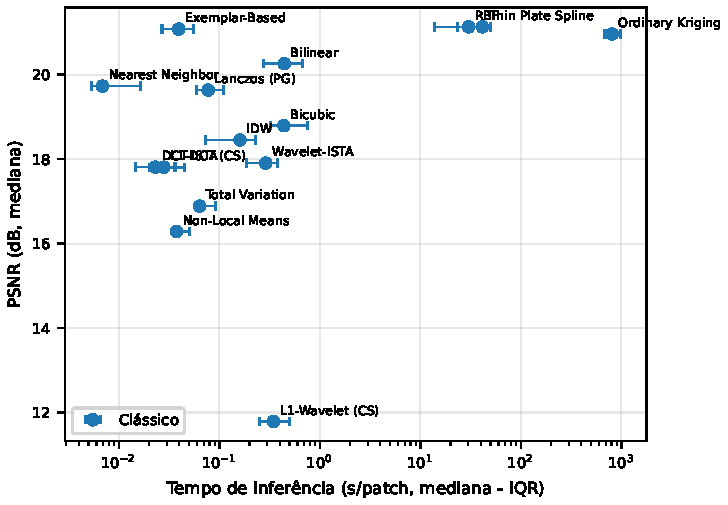
\includegraphics[width=0.78\linewidth]{figures/fig_classical_pareto}
\caption{Compromisso entre qualidade e custo de inferência para os métodos clássicos no cenário sem ruído.}
\label{fig:classical-pareto}
\end{figure*}

Do ponto de vista espectral, a \Cref{tab:spectral-rmse-classical} mostra que os métodos mais fortes no ranking global tendem a manter erro competitivo ao longo das quatro bandas analisadas.
Isso é relevante porque evita uma interpretação superficial em que PSNR global elevado mascararia erro excessivo em bandas específicas.
Os melhores métodos clássicos não aparecem fortes apenas por uma média agregada favorável.
Eles sustentam desempenho relativamente uniforme ao longo do espectro disponível.

\begin{table}[htbp]
\centering
\caption{RMSE mediano por banda (IC95\%) dos métodos clássicos por nível de ruído. Menor é melhor.}
\label{tab:spectral-rmse-classical}
\footnotesize
\resizebox{\linewidth}{!}{%
\begin{tabular}{llcccc}
\toprule
Tipo & Método & B2 (Blue) $\downarrow$ & B3 (Green) $\downarrow$ & B4 (Red) $\downarrow$ & B8 (NIR) $\downarrow$ \\
\midrule
\multicolumn{6}{l}{\textbf{Nível de ruído: Sem ruído}} \\
Clássico & Ordinary Kriging & $\mathbf{0.080_{\pm 0.016}}$ & $\mathbf{0.082_{\pm 0.015}}$ & $0.092_{\pm 0.016}$ & $0.087_{\pm 0.018}$ \\
Clássico & Exemplar-Based & \underline{$0.081_{\pm 0.019}$} & $0.083_{\pm 0.015}$ & \textit{$0.085_{\pm 0.016}$} & $\mathbf{0.086_{\pm 0.014}}$ \\
Clássico & RBF & \textit{$0.082_{\pm 0.020}$} & \underline{$0.082_{\pm 0.016}$} & $\mathbf{0.083_{\pm 0.015}}$ & \underline{$0.086_{\pm 0.016}$} \\
\midrule
\multicolumn{6}{l}{\textbf{Nível de ruído: 40 dB}} \\
Clássico & Exemplar-Based & $\mathbf{0.080_{\pm 0.018}}$ & $\mathbf{0.080_{\pm 0.015}}$ & $\mathbf{0.084_{\pm 0.015}}$ & $\mathbf{0.084_{\pm 0.014}}$ \\
Clássico & Ordinary Kriging & \underline{$0.080_{\pm 0.016}$} & $0.083_{\pm 0.015}$ & $0.091_{\pm 0.016}$ & $0.087_{\pm 0.017}$ \\
Clássico & RBF & \textit{$0.082_{\pm 0.019}$} & \underline{$0.081_{\pm 0.017}$} & \underline{$0.084_{\pm 0.015}$} & \underline{$0.086_{\pm 0.015}$} \\
\midrule
\multicolumn{6}{l}{\textbf{Nível de ruído: 30 dB}} \\
Clássico & Ordinary Kriging & $\mathbf{0.083_{\pm 0.016}}$ & \underline{$0.083_{\pm 0.015}$} & $0.092_{\pm 0.016}$ & $\mathbf{0.087_{\pm 0.016}}$ \\
Clássico & Exemplar-Based & \underline{$0.085_{\pm 0.014}$} & $\mathbf{0.083_{\pm 0.012}}$ & $\mathbf{0.087_{\pm 0.013}}$ & \underline{$0.088_{\pm 0.013}$} \\
Clássico & RBF & \textit{$0.086_{\pm 0.015}$} & \textit{$0.089_{\pm 0.015}$} & \underline{$0.089_{\pm 0.013}$} & \textit{$0.091_{\pm 0.017}$} \\
\midrule
\multicolumn{6}{l}{\textbf{Nível de ruído: 20 dB}} \\
Clássico & Ordinary Kriging & $\mathbf{0.084_{\pm 0.014}}$ & $\mathbf{0.084_{\pm 0.010}}$ & $\mathbf{0.093_{\pm 0.015}}$ & $\mathbf{0.088_{\pm 0.015}}$ \\
Clássico & Exemplar-Based & \underline{$0.101_{\pm 0.016}$} & \textit{$0.098_{\pm 0.014}$} & \underline{$0.101_{\pm 0.013}$} & \textit{$0.108_{\pm 0.013}$} \\
Clássico & Bilinear & \textit{$0.101_{\pm 0.014}$} & \underline{$0.095_{\pm 0.013}$} & \textit{$0.104_{\pm 0.014}$} & \underline{$0.101_{\pm 0.014}$} \\
\bottomrule
\end{tabular}
}
\end{table}


A \Cref{fig:classical-spectral-profile} reforça essa leitura ao resumir o RMSE mediano por banda dos principais métodos clássicos.
Visualmente, a figura mostra que métodos fracos tendem a exibir maior separação entre bandas, enquanto os mais fortes preservam perfil espectral mais compacto.
Essa regularidade sugere que a qualidade observada não é apenas radiométrica em sentido amplo, mas também espectralmente consistente.

\begin{figure}[htbp]
\centering
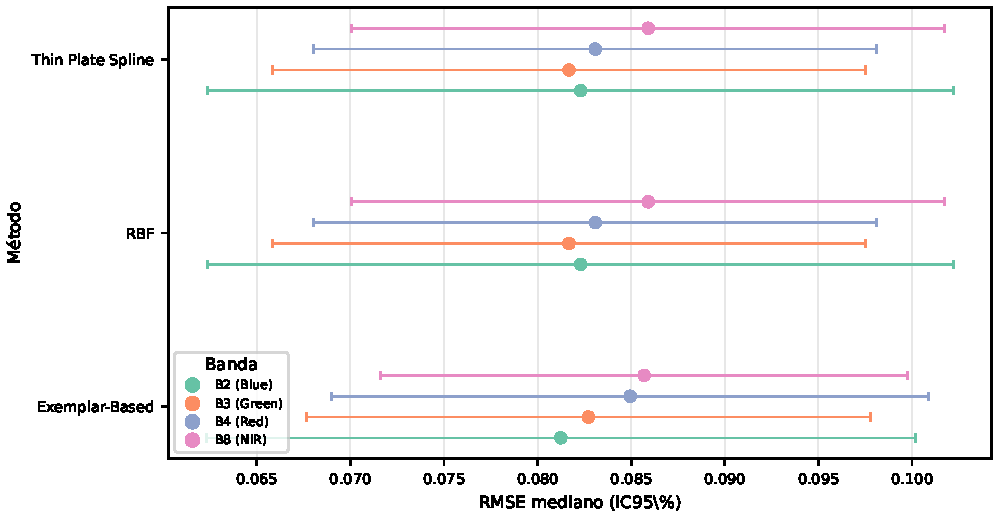
\includegraphics[width=\linewidth]{figures/fig_classical_spectral_profile}
\caption{Perfil espectral do RMSE mediano para os métodos clássicos mais competitivos no cenário sem ruído.}
\label{fig:classical-spectral-profile}
\end{figure}

O segundo eixo do bloco clássico é a robustez ao ruído.
As tabelas \Cref{tab:degradation-psnr-classical} e \Cref{tab:noise-slope-psnr-classical} mostram que qualidade absoluta e estabilidade não coincidem perfeitamente.
Métodos muito fortes em cenário limpo nem sempre apresentam a menor perda relativa quando o ruído aumenta.
Esse resultado tem implicação direta para aplicações reais, pois distingue métodos que maximizam qualidade em condição ideal daqueles que mantêm desempenho mais previsível em condição adversa.

\begin{table}[htbp]
\centering
\caption{Queda percentual no PSNR (mediana, IC95\%) (sem ruído → 20 dB) para os métodos clássicos, estratificada por faixa de entropia e janela de cálculo.}
\label{tab:degradation-psnr-classical}
\footnotesize
\resizebox{\linewidth}{!}{%
\begin{tabular}{lccc}
\toprule
Método & Baixa & Média & Alta \\
\midrule
\multicolumn{4}{l}{\textbf{Janela de entropia: 7x7}} \\
Exemplar-Based & $4.1\%_{\pm 3.645}$ & $10.8\%_{\pm 7.629}$ & $6.2\%_{\pm 4.993}$ \\
RBF & $5.8\%_{\pm 4.659}$ & $14.2\%_{\pm 7.203}$ & $8.0\%_{\pm 5.669}$ \\
Thin Plate Spline & $5.8\%_{\pm 4.659}$ & $14.2\%_{\pm 7.203}$ & $8.0\%_{\pm 5.669}$ \\
\midrule
\multicolumn{4}{l}{\textbf{Janela de entropia: 15x15}} \\
Exemplar-Based & $2.7\%_{\pm 5.677}$ & $8.2\%_{\pm 8.153}$ & $8.3\%_{\pm 7.339}$ \\
RBF & $6.1\%_{\pm 5.595}$ & $10.7\%_{\pm 7.259}$ & $8.6\%_{\pm 6.677}$ \\
Thin Plate Spline & $6.1\%_{\pm 5.595}$ & $10.7\%_{\pm 7.259}$ & $8.6\%_{\pm 6.677}$ \\
\midrule
\multicolumn{4}{l}{\textbf{Janela de entropia: 31x31}} \\
Exemplar-Based & $7.5\%_{\pm 5.544}$ & $4.2\%_{\pm 4.535}$ & $10.6\%_{\pm 8.373}$ \\
RBF & $9.9\%_{\pm 6.210}$ & $7.1\%_{\pm 5.784}$ & $12.1\%_{\pm 9.047}$ \\
Thin Plate Spline & $9.9\%_{\pm 6.210}$ & $7.1\%_{\pm 5.784}$ & $12.1\%_{\pm 9.047}$ \\
\bottomrule
\end{tabular}
}
\end{table}


\begin{table}[htbp]
\centering
\caption{Inclinação do PSNR vs ruído (20/30/40 dB, mediana, IC95\%) para os métodos clássicos, estratificada por faixa de entropia e janela de cálculo.}
\label{tab:noise-slope-psnr-classical}
\footnotesize
\resizebox{\linewidth}{!}{%
\begin{tabular}{lccc}
\toprule
Método & Baixa & Média & Alta \\
\midrule
\multicolumn{4}{l}{\textbf{Janela de entropia: 7x7}} \\
Exemplar-Based & $0.040_{\pm 0.036}$ & $0.128_{\pm 0.093}$ & $0.061_{\pm 0.051}$ \\
RBF & $0.052_{\pm 0.044}$ & $0.171_{\pm 0.092}$ & $0.084_{\pm 0.055}$ \\
Thin Plate Spline & $0.052_{\pm 0.044}$ & $0.171_{\pm 0.092}$ & $0.084_{\pm 0.055}$ \\
\midrule
\multicolumn{4}{l}{\textbf{Janela de entropia: 15x15}} \\
Exemplar-Based & $0.027_{\pm 0.064}$ & $0.096_{\pm 0.095}$ & $0.085_{\pm 0.075}$ \\
RBF & $0.060_{\pm 0.062}$ & $0.125_{\pm 0.085}$ & $0.090_{\pm 0.071}$ \\
Thin Plate Spline & $0.060_{\pm 0.062}$ & $0.125_{\pm 0.085}$ & $0.090_{\pm 0.071}$ \\
\midrule
\multicolumn{4}{l}{\textbf{Janela de entropia: 31x31}} \\
Exemplar-Based & $0.078_{\pm 0.064}$ & $0.037_{\pm 0.054}$ & $0.115_{\pm 0.095}$ \\
RBF & $0.108_{\pm 0.068}$ & $0.073_{\pm 0.060}$ & $0.132_{\pm 0.100}$ \\
Thin Plate Spline & $0.108_{\pm 0.068}$ & $0.073_{\pm 0.060}$ & $0.132_{\pm 0.100}$ \\
\bottomrule
\end{tabular}
}
\end{table}


As tabelas de robustez também mostram que a relação entre entropia e degradação não é monotônica simples.
Em várias combinações de método e janela, a faixa média de entropia se comporta de forma mais instável do que a faixa alta.
Isso sugere a existência de um regime intermediário particularmente difícil, em que a cena contém complexidade suficiente para desafiar métodos locais simples, mas ainda não oferece repetição estrutural ou regularidade global suficiente para favorecer de forma consistente abordagens mais sofisticadas.

Esse comportamento aparece de forma mais intuitiva na \Cref{fig:classical-noise-robustness}.
Os três painéis, separados por faixa de entropia na janela 15x15, mostram que a ordenação relativa entre os métodos sofre pequenas mudanças conforme o cenário se torna mais adverso.
Esses cruzamentos seriam menos visíveis em tabelas isoladas e ajudam a sustentar a ideia de que robustez ao ruído deve ser tratada como dimensão própria do problema.

\begin{figure*}[htbp]
\centering
\begin{subfigure}[t]{0.32\linewidth}
\centering
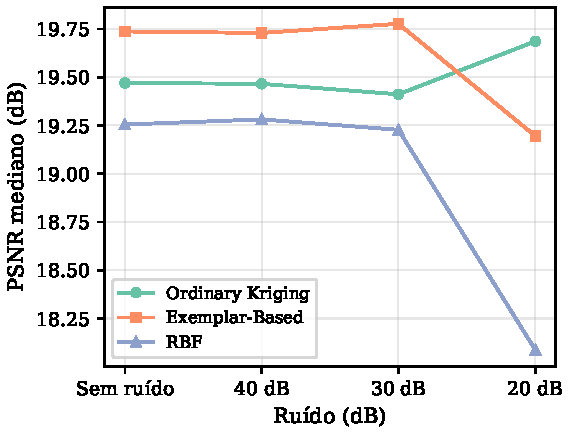
\includegraphics[width=\linewidth]{figures/fig_classical_noise_robustness_baixa}
\caption{Baixa entropia.}
\end{subfigure}
\hfill
\begin{subfigure}[t]{0.32\linewidth}
\centering
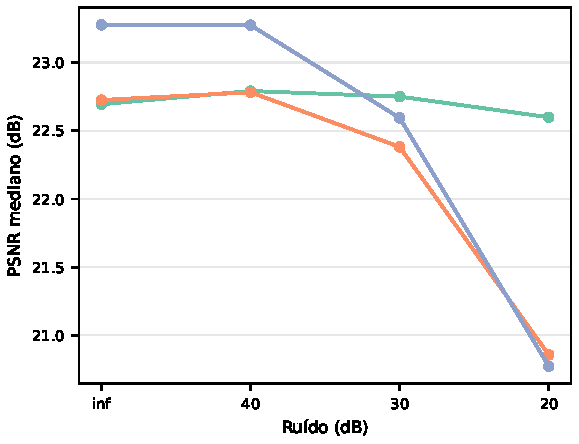
\includegraphics[width=\linewidth]{figures/fig_classical_noise_robustness_media}
\caption{Entropia média.}
\end{subfigure}
\hfill
\begin{subfigure}[t]{0.32\linewidth}
\centering
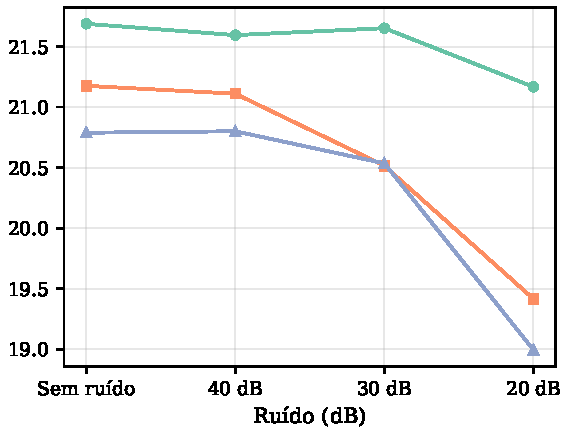
\includegraphics[width=\linewidth]{figures/fig_classical_noise_robustness_alta}
\caption{Alta entropia.}
\end{subfigure}
\caption{Robustez ao ruído dos principais métodos clássicos, resumida pelo PSNR mediano em cada faixa de entropia para a janela 15x15.}
\label{fig:classical-noise-robustness}
\end{figure*}

O terceiro eixo da análise clássica é a associação entre entropia local e qualidade de reconstrução.
Na \Cref{tab:spearman-entropy-classical-e15}, observa-se que a correlação entre entropia e desempenho varia com o método e com a métrica.
Alguns algoritmos apresentam associação fraca ou próxima de zero em PSNR, mas associação mais marcada em SSIM, SAM ou ERGAS.
Em outros casos, a direção do efeito muda conforme a escala da entropia ou o indicador analisado.

\begin{table}[htbp]
\centering
\caption{Correlação de Spearman entre entropia (15x15) e métricas de qualidade para os métodos clássicos (FDR).}
\label{tab:spearman-entropy-classical-e15}
\footnotesize
\begin{threeparttable}
\resizebox{\linewidth}{!}{%
\begin{tabular}{lcccc}
\toprule
Método & $\rho$({\scriptsize PSNR}) & $\rho$({\scriptsize SSIM}) & $\rho$({\scriptsize SAM}) & $\rho$({\scriptsize ERGAS}) \\
\midrule
Bicubic & $\approx 0$ & $-0.205^{\ddagger}$ & $-0.109^{*}$ & $-0.131^{\dagger}$ \\
Bilinear & $\approx 0$ & $-0.212^{\ddagger}$ & $-0.199^{\ddagger}$ & $-0.221^{\ddagger}$ \\
DCT-ISTA & $0.241^{\ddagger}$ & $\approx 0$ & $-0.357^{\ddagger}$ & $-0.400^{\ddagger}$ \\
Exemplar-Based & $\approx 0$ & $-0.214^{\ddagger}$ & $-0.122^{*}$ & $-0.108^{*}$ \\
IDW & $0.240^{\ddagger}$ & $\approx 0$ & $-0.347^{\ddagger}$ & $-0.388^{\ddagger}$ \\
Ordinary Kriging & $\approx 0$ & $-0.144^{\dagger}$ & $-0.229^{\ddagger}$ & $-0.248^{\ddagger}$ \\
L1-DCT (CS) & $0.241^{\ddagger}$ & $\approx 0$ & $-0.357^{\ddagger}$ & $-0.400^{\ddagger}$ \\
L1-Wavelet (CS) & $-0.184^{\ddagger}$ & $-0.272^{\ddagger}$ & $-0.299^{\ddagger}$ & $-0.197^{\ddagger}$ \\
Lanczos (PG) & $0.107^{*}$ & $-0.175^{\ddagger}$ & $-0.233^{\ddagger}$ & $-0.242^{\ddagger}$ \\
Nearest Neighbor & $\approx 0$ & $-0.216^{\ddagger}$ & $-0.198^{\ddagger}$ & $-0.212^{\ddagger}$ \\
Non-Local Means & $0.297^{\ddagger}$ & $0.203^{\ddagger}$ & $-0.390^{\ddagger}$ & $-0.421^{\ddagger}$ \\
RBF & $\approx 0$ & $-0.213^{\ddagger}$ & $-0.146^{\dagger}$ & $-0.129^{\dagger}$ \\
Thin Plate Spline & $\approx 0$ & $-0.213^{\ddagger}$ & $-0.146^{\dagger}$ & $-0.129^{\dagger}$ \\
Total Variation & $0.245^{\ddagger}$ & $\approx 0$ & $-0.360^{\ddagger}$ & $-0.377^{\ddagger}$ \\
Wavelet-ISTA & $0.234^{\ddagger}$ & $\approx 0$ & $-0.337^{\ddagger}$ & $-0.370^{\ddagger}$ \\
\bottomrule
\end{tabular}
}
\begin{tablenotes}
\scriptsize
\item $^{*}$ $p_{FDR}<0{,}05$.
\item $^{\dagger}$ $p_{FDR}<0{,}01$.
\item $^{\ddagger}$ $p_{FDR}<0{,}001$.
\end{tablenotes}
\end{threeparttable}
\end{table}


Esse resultado é conceitualmente importante porque impede uma interpretação simplificada do tipo “mais entropia implica pior reconstrução”.
O que os dados mostram é algo mais rico.
A complexidade espacial altera o regime de erro dos métodos, mas essa alteração depende da família algorítmica, do nível de ruído e da métrica que sintetiza o desempenho.
Logo, a entropia funciona melhor como variável moderadora do comportamento do método do que como marcador universal de dificuldade com direção invariável.

A \Cref{fig:classical-correlation-heatmap} sintetiza essa leitura em um único painel.
Ao reunir correlações entre múltiplas janelas de entropia e várias métricas, a figura evidencia o caráter multiescala e multi-métrica do problema.
Também chama atenção o fato de que nem todas as associações são fortes.
Isso é relevante porque mostra que a entropia local explica parte importante da variação de desempenho, mas não esgota a heterogeneidade observada entre métodos e cenas.

\begin{figure*}[htbp]
\centering
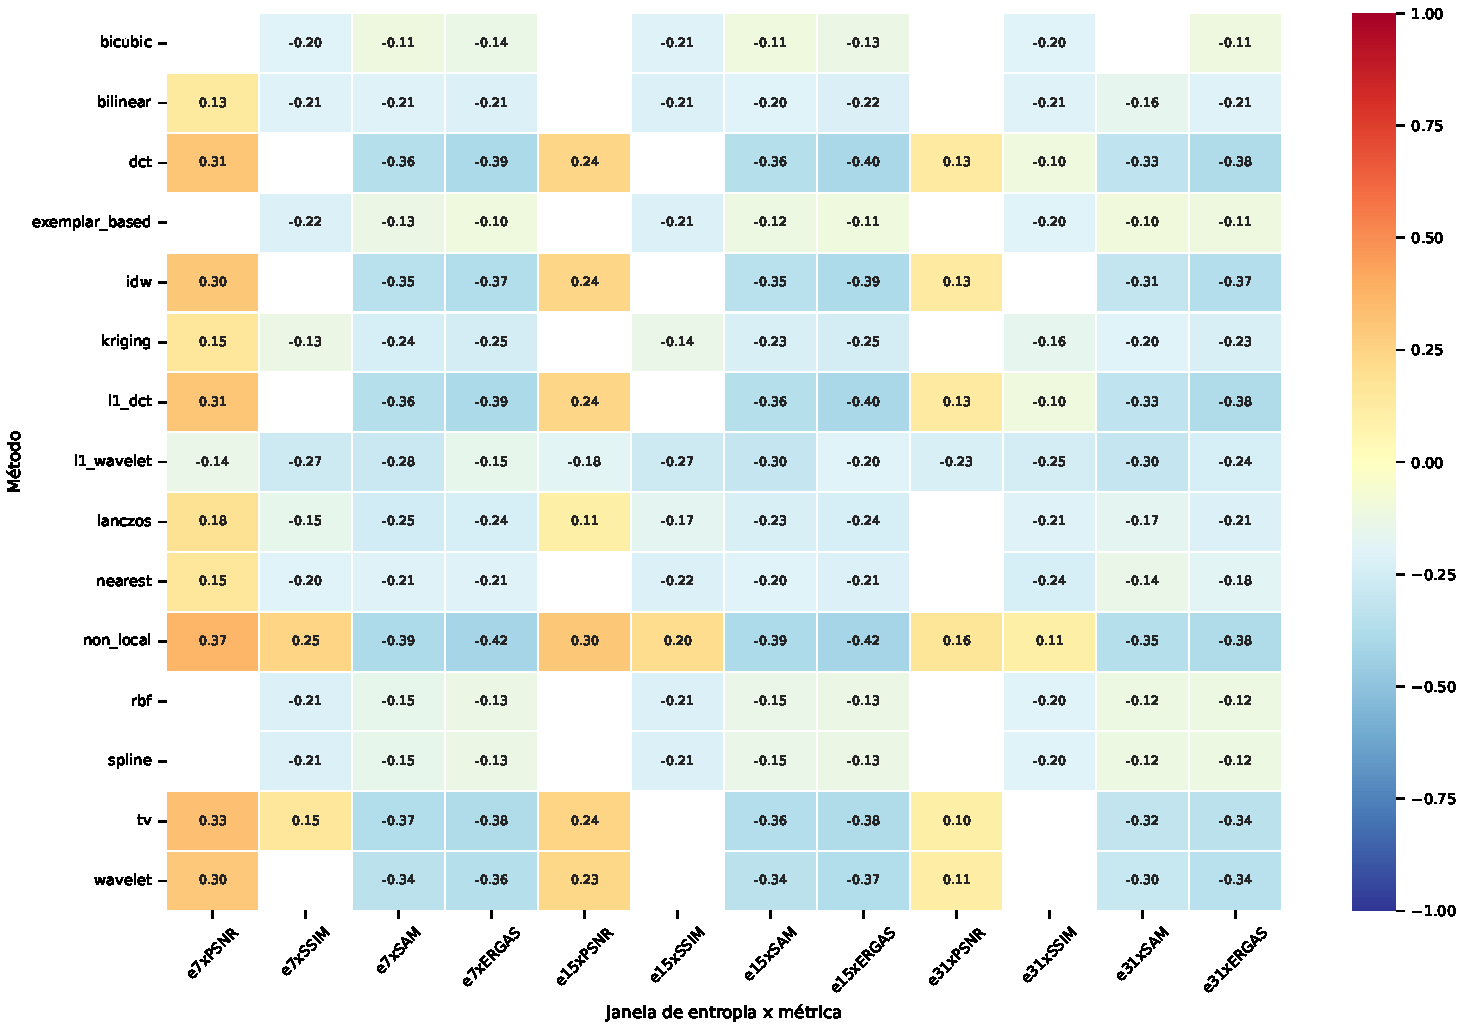
\includegraphics[width=0.90\linewidth]{figures/fig_classical_correlation_heatmap}
\caption{Mapa de correlação entre entropia local e métricas de qualidade para os métodos clássicos.}
\label{fig:classical-correlation-heatmap}
\end{figure*}

Em conjunto, o bloco clássico sustenta três conclusões centrais.
Primeiro, existe um grupo pequeno de métodos claramente superiores ao restante, mas sem dominância universal entre qualidade, custo e estabilidade.
Segundo, kriging se destaca como solução particularmente robusta em cenários mais ruidosos, enquanto RBF, spline e exemplar\_based se mostram muito fortes em qualidade absoluta sob condições menos adversas.
Terceiro, a complexidade espacial da cena altera o comportamento relativo dos métodos de forma dependente da métrica e da escala de entropia considerada.

\subsection{Resultados dos Modelos de Aprendizado Profundo}

O bloco de aprendizado profundo apresenta uma dinâmica interna distinta da observada nos métodos clássicos.
Aqui, a questão principal não é o custo extremo de inferência, mas a diferença de perfil entre arquiteturas que compartilham o mesmo domínio de avaliação.
A \Cref{tab:global-scoreboard-dl} fornece o resumo mais direto dessa comparação.

\begin{table*}[htbp]
\centering
\caption{Placar global multi-métrica dos métodos de DL por nível de ruído (mediana e IC95\%). \textbf{Negrito}: melhor por métrica dentro do grupo.}
\label{tab:global-scoreboard-dl}
\footnotesize
\resizebox{\linewidth}{!}{%
\begin{tabular}{llccccc}
\toprule
Tipo & Método & PSNR (dB) $\uparrow$ & SSIM $\uparrow$ & RMSE $\downarrow$ & SAM $\downarrow$ & ERGAS $\downarrow$ \\
\midrule
\multicolumn{7}{l}{\textbf{Nível de ruído: todos os níveis de ruído}} \\
DL & U-Net & $\mathbf{24.31_{\pm 0.126}}$ & $\mathbf{0.66_{\pm 0.004}}$ & $\mathbf{0.06_{\pm 0.001}}$ & $\mathbf{5.12_{\pm 0.073}}$ & $\mathbf{27.75_{\pm 0.332}}$ \\
DL & GAN & $23.59_{\pm 0.116}$ & $0.62_{\pm 0.004}$ & $0.07_{\pm 0.001}$ & $5.61_{\pm 0.078}$ & $29.83_{\pm 0.349}$ \\
DL & ViT & $23.50_{\pm 0.121}$ & $0.61_{\pm 0.004}$ & $0.07_{\pm 0.001}$ & $5.61_{\pm 0.079}$ & $30.17_{\pm 0.386}$ \\
\midrule
\multicolumn{7}{l}{\textbf{Nível de ruído: Sem ruído}} \\
DL & U-Net & $\mathbf{24.66_{\pm 0.140}}$ & $\mathbf{0.70_{\pm 0.005}}$ & $\mathbf{0.06_{\pm 0.001}}$ & $\mathbf{4.88_{\pm 0.068}}$ & $\mathbf{27.12_{\pm 0.344}}$ \\
DL & GAN & $23.67_{\pm 0.115}$ & $0.65_{\pm 0.005}$ & $0.07_{\pm 0.001}$ & $5.55_{\pm 0.078}$ & $29.60_{\pm 0.383}$ \\
DL & ViT & $23.56_{\pm 0.115}$ & $0.63_{\pm 0.005}$ & $0.07_{\pm 0.001}$ & $5.57_{\pm 0.081}$ & $29.96_{\pm 0.429}$ \\
\midrule
\multicolumn{7}{l}{\textbf{Nível de ruído: 40 dB}} \\
DL & U-Net & $\mathbf{24.64_{\pm 0.131}}$ & $\mathbf{0.69_{\pm 0.005}}$ & $\mathbf{0.06_{\pm 0.001}}$ & $\mathbf{4.89_{\pm 0.069}}$ & $\mathbf{27.10_{\pm 0.337}}$ \\
DL & GAN & $23.67_{\pm 0.116}$ & $0.65_{\pm 0.005}$ & $0.07_{\pm 0.001}$ & $5.56_{\pm 0.079}$ & $29.62_{\pm 0.391}$ \\
DL & ViT & $23.56_{\pm 0.110}$ & $0.63_{\pm 0.005}$ & $0.07_{\pm 0.001}$ & $5.57_{\pm 0.080}$ & $29.95_{\pm 0.435}$ \\
\midrule
\multicolumn{7}{l}{\textbf{Nível de ruído: 30 dB}} \\
DL & U-Net & $\mathbf{24.52_{\pm 0.140}}$ & $\mathbf{0.68_{\pm 0.004}}$ & $\mathbf{0.06_{\pm 0.001}}$ & $\mathbf{4.99_{\pm 0.069}}$ & $\mathbf{27.40_{\pm 0.322}}$ \\
DL & GAN & $23.63_{\pm 0.117}$ & $0.64_{\pm 0.004}$ & $0.07_{\pm 0.001}$ & $5.58_{\pm 0.084}$ & $29.71_{\pm 0.364}$ \\
DL & ViT & $23.52_{\pm 0.123}$ & $0.62_{\pm 0.005}$ & $0.07_{\pm 0.001}$ & $5.58_{\pm 0.078}$ & $30.04_{\pm 0.389}$ \\
\midrule
\multicolumn{7}{l}{\textbf{Nível de ruído: 20 dB}} \\
DL & U-Net & $\mathbf{23.58_{\pm 0.114}}$ & $\mathbf{0.58_{\pm 0.003}}$ & $\mathbf{0.07_{\pm 0.001}}$ & $\mathbf{5.69_{\pm 0.065}}$ & $\mathbf{29.46_{\pm 0.358}}$ \\
DL & ViT & $23.34_{\pm 0.138}$ & $0.56_{\pm 0.004}$ & $0.07_{\pm 0.001}$ & $5.70_{\pm 0.083}$ & $30.55_{\pm 0.348}$ \\
DL & GAN & $23.34_{\pm 0.126}$ & $0.57_{\pm 0.004}$ & $0.07_{\pm 0.001}$ & $5.73_{\pm 0.073}$ & $30.29_{\pm 0.399}$ \\
\bottomrule
\end{tabular}
}
\end{table*}


A tabela mostra que U-Net domina a qualidade absoluta de forma consistente.
Ela lidera em PSNR, SSIM, RMSE, SAM e ERGAS em todos os níveis de ruído considerados, o que indica forte equilíbrio entre fidelidade radiométrica, preservação estrutural e coerência espectral.
Esse resultado sugere que as conexões de atalho e a propagação multiescala de contexto continuam sendo uma estratégia muito eficaz para reconstrução de lacunas no domínio Sentinel-2.

GAN e ViT formam um segundo patamar relativamente próximo entre si.
Eles não alcançam a qualidade absoluta da U-Net, mas também não colapsam para o nível de AE e VAE.
Isso sugere que tanto a modelagem adversarial quanto a atenção conseguem capturar regularidades importantes do problema, embora ainda não superem a vantagem arquitetural oferecida pela combinação de codificação multiescala e skip connections.
AE e VAE, por sua vez, mantêm papel analítico importante como baselines de gargalo latente, mostrando que compressão simples do contexto observado não é suficiente para atingir o melhor nível de fidelidade.

Em termos de custo, a \Cref{tab:runtime-speed-dl} revela um cenário diferente do bloco clássico.
Embora existam diferenças entre arquiteturas, todas permanecem em uma faixa operacional muito mais favorável do que os métodos clássicos mais pesados.
AE e VAE aparecem como os modelos mais rápidos e com melhor relação PSNR/s, enquanto U-Net cobra um custo adicional em troca de qualidade superior.
Esse custo, porém, é marginal quando comparado ao salto de tempo observado entre os clássicos de alto custo e os demais métodos.

\begin{table}[htbp]
\centering
\caption{Velocidade e viabilidade prática dos métodos de DL no cenário sem ruído. PSNR/s indica eficiência. Hardware: Rocky Linux 9.5, NVIDIA A100 80GB PCIe, driver 550.90.07, CUDA 12.4/12.6.2.}
\label{tab:runtime-speed-dl}
\footnotesize
\resizebox{\linewidth}{!}{%
\begin{tabular}{llccc}
\toprule
Tipo & Método & PSNR (dB) $\uparrow$ & Tempo (s/patch) $\downarrow$ & PSNR/s $\uparrow$ \\
\midrule
DL & VAE & $23.05$ & $0.0034$ & $\mathbf{6772.2}$ \\
DL & GAN & \underline{$23.63$} & $0.0036$ & \underline{$6506.7$} \\
DL & AE & $22.86$ & $0.0035$ & \textit{$6473.7$} \\
DL & ViT & \textit{$23.42$} & $0.0042$ & $5604.4$ \\
DL & U-Net & $\mathbf{24.56}$ & $0.0055$ & $4480.6$ \\
\bottomrule
\end{tabular}
}
\end{table}


Essa distinção muda a interpretação prática do ranking.
No bloco de aprendizado profundo, a discussão de eficiência diz respeito principalmente ao preço marginal pago por qualidade adicional.
No bloco clássico, por outro lado, a discussão frequentemente separa métodos viáveis de métodos muito caros.
Isso ajuda a entender por que a U-Net continua sendo atraente mesmo não liderando em velocidade.
O ganho absoluto de qualidade é suficientemente alto para justificar o custo extra em muitas aplicações.

A \Cref{fig:dl-comparison} sintetiza esse padrão comparando os modelos no cenário \texttt{entropy\_all}.
Visualmente, a figura reforça que a superioridade da U-Net não está restrita a uma única métrica.
O modelo aparece consistentemente forte em critérios complementares, o que reduz a chance de sua liderança ser artefato de um único indicador.

\begin{figure*}[htbp]
\centering
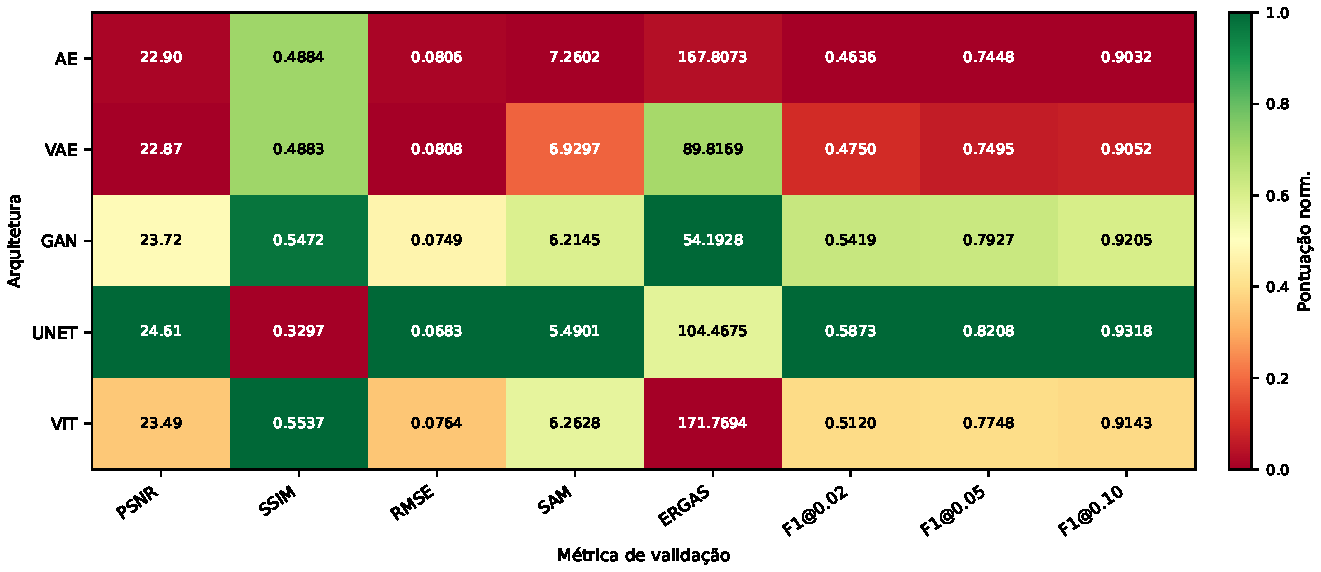
\includegraphics[width=0.82\linewidth]{figures/fig_dl_comparison}
\caption{Comparação interna entre arquiteturas de aprendizado profundo no cenário \texttt{entropy\_all}.}
\label{fig:dl-comparison}
\end{figure*}

O segundo eixo do bloco de \gls{DL} é a robustez ao ruído.
As tabelas \Cref{tab:degradation-psnr-dl} e \Cref{tab:noise-slope-psnr-dl} mostram que a liderança absoluta da U-Net não implica dominância completa em estabilidade relativa.
GAN e ViT frequentemente exibem menor degradação percentual em vários cenários, mesmo permanecendo abaixo da U-Net em valor absoluto de PSNR.

\begin{table}[htbp]
\centering
\caption{Queda percentual no PSNR (mediana, IC95\%) (sem ruído → 20 dB) para os métodos de DL, estratificada por faixa de entropia e janela de cálculo.}
\label{tab:degradation-psnr-dl}
\footnotesize
\resizebox{\linewidth}{!}{%
\begin{tabular}{lccc}
\toprule
Método & Baixa & Média & Alta \\
\midrule
\multicolumn{4}{l}{\textbf{Janela de entropia: 7x7}} \\
U-Net & $5.1\%_{\pm 0.593}$ & $5.0\%_{\pm 0.558}$ & $3.4\%_{\pm 0.628}$ \\
GAN & $1.2\%_{\pm 0.506}$ & $1.4\%_{\pm 0.456}$ & $1.2\%_{\pm 0.476}$ \\
ViT & $0.6\%_{\pm 0.330}$ & $0.7\%_{\pm 0.375}$ & $0.6\%_{\pm 0.369}$ \\
\midrule
\multicolumn{4}{l}{\textbf{Janela de entropia: 15x15}} \\
U-Net & $4.4\%_{\pm 0.590}$ & $4.6\%_{\pm 0.632}$ & $4.4\%_{\pm 0.716}$ \\
GAN & $1.0\%_{\pm 0.484}$ & $1.3\%_{\pm 0.492}$ & $1.3\%_{\pm 0.482}$ \\
ViT & $0.7\%_{\pm 0.398}$ & $0.7\%_{\pm 0.333}$ & $0.9\%_{\pm 0.435}$ \\
\midrule
\multicolumn{4}{l}{\textbf{Janela de entropia: 31x31}} \\
U-Net & $3.7\%_{\pm 0.524}$ & $3.9\%_{\pm 0.478}$ & $5.4\%_{\pm 0.742}$ \\
GAN & $0.7\%_{\pm 0.435}$ & $1.1\%_{\pm 0.429}$ & $1.7\%_{\pm 0.507}$ \\
ViT & $0.6\%_{\pm 0.370}$ & $0.7\%_{\pm 0.270}$ & $0.9\%_{\pm 0.479}$ \\
\bottomrule
\end{tabular}
}
\end{table}


\begin{table}[htbp]
\centering
\caption{Inclinação do PSNR vs ruído (20/30/40 dB, mediana, IC95\%) para os métodos de DL, estratificada por faixa de entropia e janela de cálculo.}
\label{tab:noise-slope-psnr-dl}
\footnotesize
\resizebox{\linewidth}{!}{%
\begin{tabular}{lccc}
\toprule
Método & Baixa & Média & Alta \\
\midrule
\multicolumn{4}{l}{\textbf{Janela de entropia: 7x7}} \\
U-Net & $0.067_{\pm 0.008}$ & $0.062_{\pm 0.008}$ & $0.039_{\pm 0.007}$ \\
GAN & $0.017_{\pm 0.006}$ & $0.016_{\pm 0.006}$ & $0.013_{\pm 0.005}$ \\
ViT & $0.007_{\pm 0.004}$ & $0.009_{\pm 0.004}$ & $0.006_{\pm 0.004}$ \\
\midrule
\multicolumn{4}{l}{\textbf{Janela de entropia: 15x15}} \\
U-Net & $0.059_{\pm 0.008}$ & $0.058_{\pm 0.008}$ & $0.048_{\pm 0.008}$ \\
GAN & $0.012_{\pm 0.006}$ & $0.014_{\pm 0.006}$ & $0.014_{\pm 0.006}$ \\
ViT & $0.009_{\pm 0.005}$ & $0.008_{\pm 0.004}$ & $0.009_{\pm 0.005}$ \\
\midrule
\multicolumn{4}{l}{\textbf{Janela de entropia: 31x31}} \\
U-Net & $0.049_{\pm 0.007}$ & $0.048_{\pm 0.006}$ & $0.059_{\pm 0.009}$ \\
GAN & $0.009_{\pm 0.006}$ & $0.013_{\pm 0.005}$ & $0.018_{\pm 0.006}$ \\
ViT & $0.008_{\pm 0.005}$ & $0.008_{\pm 0.003}$ & $0.010_{\pm 0.005}$ \\
\bottomrule
\end{tabular}
}
\end{table}


Essa diferença é relevante porque explicita a tensão entre nível final de qualidade e sensibilidade do desempenho ao aumento de ruído.
Um modelo pode partir de um patamar mais alto e ainda assim perder mais, em termos relativos, quando a condição experimental piora.
Logo, a arquitetura mais precisa não é necessariamente a mais estável.
Para aplicações em que previsibilidade sob degradação importa tanto quanto qualidade final, essa distinção muda o critério de escolha.

A \Cref{fig:dl-noise-robustness} resume esse comportamento ao longo dos quatro níveis de ruído.
As curvas mostram que U-Net permanece à frente em termos absolutos, mas também deixam visível que as inclinações não são idênticas entre arquiteturas.
GAN e ViT preservam parte do desempenho relativo de forma mais estável, enquanto AE e VAE ocupam um regime inferior, porém regular.

\begin{figure}[htbp]
\centering
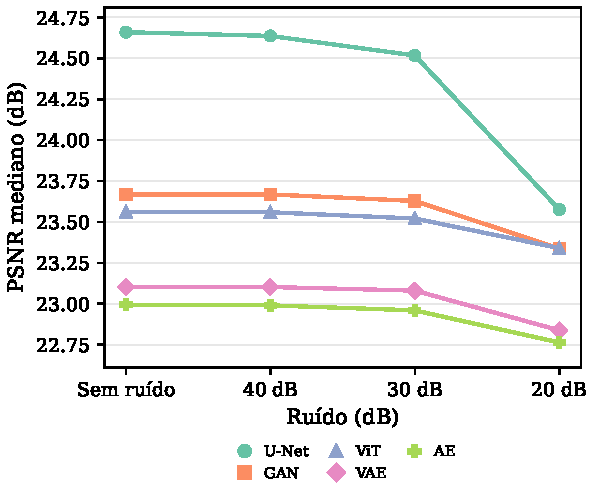
\includegraphics[width=\linewidth]{figures/fig_dl_noise_robustness}
\caption{Robustez ao ruído dos principais modelos de aprendizado profundo no cenário \texttt{entropy\_all}.}
\label{fig:dl-noise-robustness}
\end{figure}

No que diz respeito à relação entre entropia e qualidade, a \Cref{tab:spearman-entropy-dl-e15} mostra um padrão mais uniforme do que o observado no bloco clássico.
As correlações entre entropia e PSNR ou SSIM tendem a ser mais claramente negativas para a maioria das arquiteturas, sugerindo que o aumento de complexidade espacial atua como fator de dificuldade relativamente consistente dentro do conjunto de modelos profundos analisado.

\begin{table}[htbp]
\centering
\caption{Correlação de Spearman entre entropia (15x15) e métricas de qualidade para os métodos de DL (FDR).}
\label{tab:spearman-entropy-dl-e15}
\footnotesize
\begin{threeparttable}
\resizebox{\linewidth}{!}{%
\begin{tabular}{lcccc}
\toprule
Método & $\rho$({\scriptsize PSNR}) & $\rho$({\scriptsize SSIM}) & $\rho$({\scriptsize SAM}) & $\rho$({\scriptsize ERGAS}) \\
\midrule
ae & $-0.391^{\ddagger}$ & $-0.444^{\ddagger}$ & $\approx 0$ & $-0.193^{\ddagger}$ \\
gan & $-0.407^{\ddagger}$ & $-0.450^{\ddagger}$ & $\approx 0$ & $-0.129^{\ddagger}$ \\
unet & $-0.408^{\ddagger}$ & $-0.419^{\ddagger}$ & $\approx 0$ & $-0.126^{\ddagger}$ \\
vae & $-0.409^{\ddagger}$ & $-0.504^{\ddagger}$ & $\approx 0$ & $-0.176^{\ddagger}$ \\
vit & $-0.393^{\ddagger}$ & $-0.444^{\ddagger}$ & $\approx 0$ & $-0.147^{\ddagger}$ \\
\bottomrule
\end{tabular}
}
\begin{tablenotes}
\scriptsize
\item $^{*}$ $p_{FDR}<0{,}05$.
\item $^{\dagger}$ $p_{FDR}<0{,}01$.
\item $^{\ddagger}$ $p_{FDR}<0{,}001$.
\end{tablenotes}
\end{threeparttable}
\end{table}


Esse resultado é interessante porque diferencia os dois blocos do artigo.
Nos métodos clássicos, a entropia reorganiza o comportamento dos algoritmos de forma bastante heterogênea.
Nos modelos de \gls{DL}, a direção do efeito tende a ser mais estável, ainda que a magnitude varie entre arquiteturas.
Uma leitura plausível é que o treinamento supervisionado leva os modelos a internalizar um padrão mais uniforme de dificuldade associado à estrutura espacial da cena.

Em síntese, o bloco de aprendizado profundo sustenta três conclusões principais.
Primeiro, U-Net é a melhor arquitetura em qualidade absoluta no domínio avaliado.
Segundo, essa liderança não implica melhor robustez relativa em todos os cenários, já que GAN e ViT exibem degradação percentual menor em várias condições.
Terceiro, AE e VAE permanecem úteis como referências eficientes e simples, mas não alcançam o mesmo nível de fidelidade das arquiteturas mais expressivas.

\subsection{Síntese dos Achados Empíricos}

Quando os dois blocos são observados em conjunto, o resultado mais importante do artigo não é a produção de um ranking universal entre todas as técnicas.
O resultado mais importante é a demonstração de que o desempenho em preenchimento de lacunas depende do regime analítico adotado.
No bloco clássico, a principal tensão é entre qualidade alta, robustez ao ruído e custo computacional.
No bloco de aprendizado profundo, a principal tensão é entre qualidade absoluta, estabilidade relativa e perfil arquitetural.

Isso significa que a melhor escolha metodológica depende da pergunta prática que se quer responder.
Se a prioridade recai sobre métodos clássicos interpretáveis com forte análise multicritério, kriging, RBF, spline e exemplar\_based aparecem como candidatos centrais, cada um com vantagens e limitações específicas.
Se a prioridade recai sobre melhor qualidade absoluta no domínio Sentinel-2, a U-Net emerge como solução mais forte.
Se o foco se desloca para estabilidade relativa ou eficiência dentro do bloco de \gls{DL}, a decisão torna-se mais plural e abre espaço para GAN, ViT, AE e VAE conforme o objetivo operacional.
